\documentclass[letterpaper,11pt]{article}
\usepackage{graphicx}
\usepackage{listings}
\usepackage[super]{nth}
\usepackage[hyphens]{url}
\usepackage{hyperref}
\usepackage{amsmath}
\usepackage[makeroom]{cancel}
\usepackage[table]{xcolor}
\usepackage{comment}
\usepackage[space]{grffile}
\usepackage{csvsimple}
\usepackage{longtable}
\usepackage{adjustbox}


\newcommand*{\srcPath}{../src}%

\lstset{
	basicstyle=\footnotesize,
	breaklines=true,
}

\begin{document}

\begin{titlepage}

\begin{center}

\Huge{Assignment 5}

\Large{CS 734:  Introduction to Information Retrieval}

\Large{Fall 2017}

\Large{Grant Atkins}

\Large Finished on \today

\end{center}

\end{titlepage}

\newpage


% =================================
% First question
% =================================
\section*{1}

\subsection*{Question}

\begin{verbatim}

\end{verbatim}

\subsection*{Answer}


%\begin{figure}[h]
%\centering
%
\includegraphics[scale=0.4]{sitesearch.png}
%\caption{Site search example in google}
%\label{fig:sitesearch}
%\end{figure}


\clearpage

% =================================
% Second question
% =================================
\section*{2}

\subsection*{Question}

\begin{verbatim}
10.6. Find two examples of document filtering systems 
on the Web. How do they build a profile for your
information need? Is the system static or adaptive?
\end{verbatim}

\subsection*{Answer}

Two examples of document filtering systems on the web are Amazon and Medium.
When buying tech accessories such as HDMI cables, keyboards, or mouses I usually go to Amazon.
Amazon keeps track of the things I browse as well as what I previously bought and attempts to make recommendations as shown in Figure \ref{fig:ama}.
This kind of filtering is an adaptive system.
If I start looking at a specific book frequently, Amazon will eventually start recommending the same book if I haven't bought it, or books that are similar to the one I viewed.

\begin{figure}[h]
\centering

\includegraphics[scale=0.4]{amazon.png}
\caption{Amazon recommended buys}
\label{fig:ama}
\end{figure}

Another example of a document filtering system is Medium, a popular article sharing website much like blogspot.
I often enjoy reading tech related articles for machine learning, javascript, and much more on Medium.
Medium keeps track of users viewing history and then when a user visits the home page of the website it offers them lists of articles to read.
It has a ``You might like'' section where for each article it even says ``Based on your interests.''
This shows that it has filtering in place that is adaptive to my viewing history and tries to find the best trending/matching documents for my reading.
My results are shown in Figure \ref{fig:med}.
If I decide to start reading other topics a majority of the time then this filtering system will be updated over time on its own.

\begin{figure}[h]
\centering

\includegraphics[scale=0.4]{medium.png}
\caption{Medium recommended reads}
\label{fig:med}
\end{figure}

% \lstinputlisting[frame=single,caption={Sitemap created from my assignment 1 (A1) directory},label=lst:sitemap_output,captionpos=b,numbers=left,showspaces=false,showstringspaces=false,basicstyle=\footnotesize]{\srcPath/data/sitemap.xml}

\clearpage

% =================================
% 3rd question
% =================================

\section*{3}

\subsection*{Question}

\begin{verbatim}
10.11. Suggest how the maximum and minimum resource 
ranking scores, Rmax and Rmin, could be estimated 
for a given query
\end{verbatim}

\subsection*{Answer}


\clearpage

% =================================
% 4th question
% =================================

\section*{4}

\subsection*{Question}

\begin{verbatim}
11.5. How many papers dealing with term dependency 
can you find in the SIGIR proceedings since 2000?
List their citations
\end{verbatim}

\subsection*{Answer}

To solve this problem I decided to use google scholar to find the citations.
I searched on the terms ``term dependency,'' ``term dependencies,'' and ``term dependent'' with ACM SIGIR as the source and all publication later than 2000.
For this query I got 129 results as shown in Figure \ref{fig:sigir}.
Whats interesting is when I went back later this result changed going up to 155 related articles, but regardless I kept what I originally had.

Google creates a query string that I could reuse to perform these queries, for example:

\url{https://scholar.google.com/scholar?start=0&q=\%22term+dependency\%22+\%7C+\%22term+dependencies\%22+\%7C+\%22term+dependent\%22+source:\%22ACM+SIGIR\%22&hl=en&as_sdt=0,47&as_ylo=2000}

One of the keys is ``start'' indicating an offset position for pagination.
Since there were 10 results per page I created two scripts to download each page and then parse the results.
The first script I wrote was done in nodejs using headless chrome, puppeteer.js, as shown in Listing \ref{lst:head}.
The pages downloaded pages are found in my assignment 5 github repository \cite{github}.
The other script was used to parse the document for titles, citation counts, and author names as shown in Listing \ref{lst:parse}.
For this question I left out author names as it was difficult to parse utf-8 for latex.

The results are as follows:

\begin{center}
\begin{longtable}{|*2{p{3.5cm}| }}
\hline
\textbf{Title} & \textbf{Citations} \\ \hline 
A Markov random field model for term dependencies & 776 \\ \hline
Incorporating term dependency in the DFR framework & 56 \\ \hline
Modeling higher-order term dependencies in information retrieval using query hypergraphs & 54 \\ \hline
Incorporating query term dependencies in language models for document retrieval & 19 \\ \hline
Modeling term dependencies with quantum language models for IR & 21 \\ \hline
Refining term weights of documents using term dependencies & 9 \\ \hline
Score-safe term-dependency processing with hybrid indexes & 10 \\ \hline
Utilizing phrase based semantic information for term dependency & 0 \\ \hline
Automatic P hrase Indexing for Document Retrieval: An Examination of Syntactic and Non-Syntactic Methods & 169 \\ \hline
Improving Search using Proximity-Based Statistics & 1 \\ \hline
Two-stage query segmentation for information retrieval & 49 \\ \hline
Dependence language model for information retrieval & 294 \\ \hline
Random walk term weighting for information retrieval & 35 \\ \hline
A comparison of various approaches for using probabilistic dependencies in language modeling & 16 \\ \hline
Latent concept expansion using markov random fields & 226 \\ \hline
Word embedding based generalized language model for information retrieval & 49 \\ \hline
Blog track research at TREC & 56 \\ \hline
Improving weak ad-hoc queries using wikipedia asexternal corpus & 103 \\ \hline
Modelling term dependence with copulas & 8 \\ \hline
A study of Poisson query generation model for information retrieval & 52 \\ \hline
A Markov random field model for term dependencies & 776 \\ \hline
Incorporating term dependency in the DFR framework & 56 \\ \hline
Modeling higher-order term dependencies in information retrieval using query hypergraphs & 54 \\ \hline
Incorporating query term dependencies in language models for document retrieval & 19 \\ \hline
Modeling term dependencies with quantum language models for IR & 21 \\ \hline
Refining term weights of documents using term dependencies & 9 \\ \hline
Score-safe term-dependency processing with hybrid indexes & 10 \\ \hline
Utilizing phrase based semantic information for term dependency & 0 \\ \hline
Automatic P hrase Indexing for Document Retrieval: An Examination of Syntactic and Non-Syntactic Methods & 169 \\ \hline
Improving Search using Proximity-Based Statistics & 1 \\ \hline
Robust ranking models via risk-sensitive optimization & 41 \\ \hline
An unsupervised topic segmentation model incorporating word order & 28 \\ \hline
Extending BM25 with multiple query operators & 14 \\ \hline
Taily: shard selection using the tail of score distributions & 31 \\ \hline
Sentiment diversification with different biases & 19 \\ \hline
An IR-based evaluation framework for web search query segmentation & 15 \\ \hline
To index or not to index: time-space trade-offs in search engines with positional ranking functions & 17 \\ \hline
Leveraging user interaction signals for web image search & 5 \\ \hline
Query representation for cross-temporal information retrieval & 5 \\ \hline
User variability and IR system evaluation & 27 \\ \hline
Ranking document clusters using markov random fields & 13 \\ \hline
Timestamp-based result cache invalidation for web search engines & 27 \\ \hline
Pseudo test collections for training and tuning microblog rankers & 17 \\ \hline
Terms over LOAD: Leveraging Named Entities for Cross-Document Extraction and Summarization of Events & 9 \\ \hline
Query-performance prediction: setting the expectations straight & 6 \\ \hline
A context-aware time model for web search & 18 \\ \hline
Optimizing positional index structures for versioned document collections & 9 \\ \hline
Learning for Efficient Supervised Query Expansion via Two-stage Feature Selection & 2 \\ \hline
[PDF][PDF] Introduction to Probabilistic Models for Information Retrieval & 4 \\ \hline
Finding topic words for hierarchical summarization & 219 \\ \hline
A comparison of sentence retrieval techniques & 30 \\ \hline
Beyond bags of words: Effectively modeling dependence and features in information retrieval & 4 \\ \hline
MRF based approach for sentence retrieval & 6 \\ \hline
Integrating word relationships into language models & 184 \\ \hline
Social annotation in query expansion: a machine learning approach & 39 \\ \hline
The seventeenth australasian document computing symposium & 0 \\ \hline
An exploration of proximity measures in information retrieval & 245 \\ \hline
A proximity language model for information retrieval & 69 \\ \hline
Structured retrieval for question answering & 106 \\ \hline
Exploiting term dependence while handling negation in medical search & 21 \\ \hline
Positional language models for information retrieval & 198 \\ \hline
Parameterized concept weighting in verbose queries & 100 \\ \hline
The role of knowledge in conceptual retrieval: a study in the domain of clinical medicine & 73 \\ \hline
Fielded sequential dependence model for ad-hoc entity retrieval in the web of data & 33 \\ \hline
Looking inside the box: Context-sensitive translation for cross-language information retrieval & 16 \\ \hline
Embedding-based Query Expansion for Weighted Sequential Dependence Retrieval Model & 0 \\ \hline
Integrating phrase inseparability in phrase-based model & 10 \\ \hline
A support vector method for optimizing average precision & 591 \\ \hline
Modeling multi-query retrieval tasks using density matrix transformation & 4 \\ \hline
Empirical development of an exponential probabilistic model for text retrieval: using textual analysis to build a better model & 25 \\ \hline
Building a web test collection using social media & 3 \\ \hline
Improving the estimation of relevance models using large external corpora & 191 \\ \hline
Discovering key concepts in verbose queries & 262 \\ \hline
Building and applying a concept hierarchy representation of a user profile & 80 \\ \hline
An improved markov random field model for supporting verbose queries & 56 \\ \hline
CRTER: using cross terms to enhance probabilistic information retrieval & 32 \\ \hline
Parameterized fielded term dependence models for ad-hoc entity retrieval from knowledge graph & 10 \\ \hline
Query term ranking based on dependency parsing of verbose queries & 28 \\ \hline
The score-distributional threshold optimization for adaptive binary classification tasks & 69 \\ \hline
Learning to reweight terms with distributed representations & 35 \\ \hline
Building simulated queries for known-item topics: an analysis using six european languages & 97 \\ \hline
Unsupervised query segmentation using clickthrough for information retrieval & 46 \\ \hline
Compact query term selection using topically related text & 38 \\ \hline
A frequency-based and a poisson-based definition of the probability of being informative & 39 \\ \hline
Positional relevance model for pseudo-relevance feedback & 161 \\ \hline
Learning for search result diversification & 42 \\ \hline
Exploring reductions for long web queries & 74 \\ \hline
Using statistical decision theory and relevance models for query-performance prediction & 25 \\ \hline
Exploiting semantics for improving clinical information retrieval & 21 \\ \hline
Modeling subset distributions for verbose queries & 11 \\ \hline
Axiomatic analysis for improving the log-logistic feedback model & 8 \\ \hline
Topic-centric classification of twitter user's political orientation & 12 \\ \hline
Sigir 2014 workshop on semantic matching in information retrieval & 4 \\ \hline
Discriminative models for information retrieval & 314 \\ \hline
Retrieval and feedback models for blog feed search & 150 \\ \hline
A ranking approach to target detection for automatic link generation & 9 \\ \hline
Flat vs. hierarchical phrase-based translation models for cross-language information retrieval & 3 \\ \hline
Non-compositional term dependence for information retrieval & 7 \\ \hline
Query performance prediction in web search environments & 169 \\ \hline
Building enriched document representations using aggregated anchor text & 62 \\ \hline
How good is a span of terms?: exploiting proximity to improve web retrieval & 47 \\ \hline
Query expansion using path-constrained random walks & 25 \\ \hline
An adaptive evidence weighting method for medical record search & 14 \\ \hline
Learning to efficiently rank & 74 \\ \hline
Exploiting proximity feature in bigram language model for information retrieval & 6 \\ \hline
Efficient cost-aware cascade ranking in multi-stage retrieval & 3 \\ \hline
Set-based model: A new approach for information retrieval & 38 \\ \hline
Modeling click-through based word-pairs for web search & 3 \\ \hline
Term Proximity Constraints for Pseudo-Relevance Feedback & 0 \\ \hline
Improving language estimation with the paragraph vector model for ad-hoc retrieval & 15 \\ \hline
Learning to respond with deep neural networks for retrieval-based human-computer conversation system & 31 \\ \hline
Find-similar: similarity browsing as a search tool & 55 \\ \hline
Linear discriminant model for information retrieval & 118 \\ \hline
Quote Recommendation in Dialogue using Deep Neural Network & 2 \\ \hline
Query term ranking based on search results overlap & 1 \\ \hline
Document retrieval using entity-based language models & 15 \\ \hline
Modeling Document Novelty with Neural Tensor Network for Search Result Diversification & 10 \\ \hline
An enhanced context-sensitive proximity model for probabilistic information retrieval & 6 \\ \hline
Efficient \& Effective Selective Query Rewriting with Efficiency Predictions & 0 \\ \hline
A Probabilistic Model for Information Retrieval Based on Maximum Value Distribution & 3 \\ \hline
Using key concepts in a translation model for retrieval & 8 \\ \hline
Evaluating non-deterministic retrieval systems & 3 \\ \hline
A simple enhancement for ad-hoc information retrieval via topic modelling & 4 \\ \hline
Retrieval sensitivity under training using different measures & 14 \\ \hline
Copulas for information retrieval & 19 \\ \hline
DBpedia-Entity v2: A Test Collection for Entity Search & 1 \\ \hline
On the cost of phrase-based ranking & 1 \\ \hline
SPOT: Selecting occuPations frOm Trajectories & 0 \\ \hline
Entity query feature expansion using knowledge base links & 84 \\ \hline
\end{longtable}
\end{center}

 \lstinputlisting[frame=single,caption={Headless chrome script to download rendered pages},label=lst:head,captionpos=b,numbers=left,showspaces=false,showstringspaces=false,basicstyle=\footnotesize]{\srcPath/headless.js}

 \lstinputlisting[frame=single,caption={Script to parse google scholar HTML pages},label=lst:parse,captionpos=b,numbers=left,showspaces=false,showstringspaces=false,basicstyle=\footnotesize]{\srcPath/parse_scholar.py}


\begin{figure}[h]
\centering
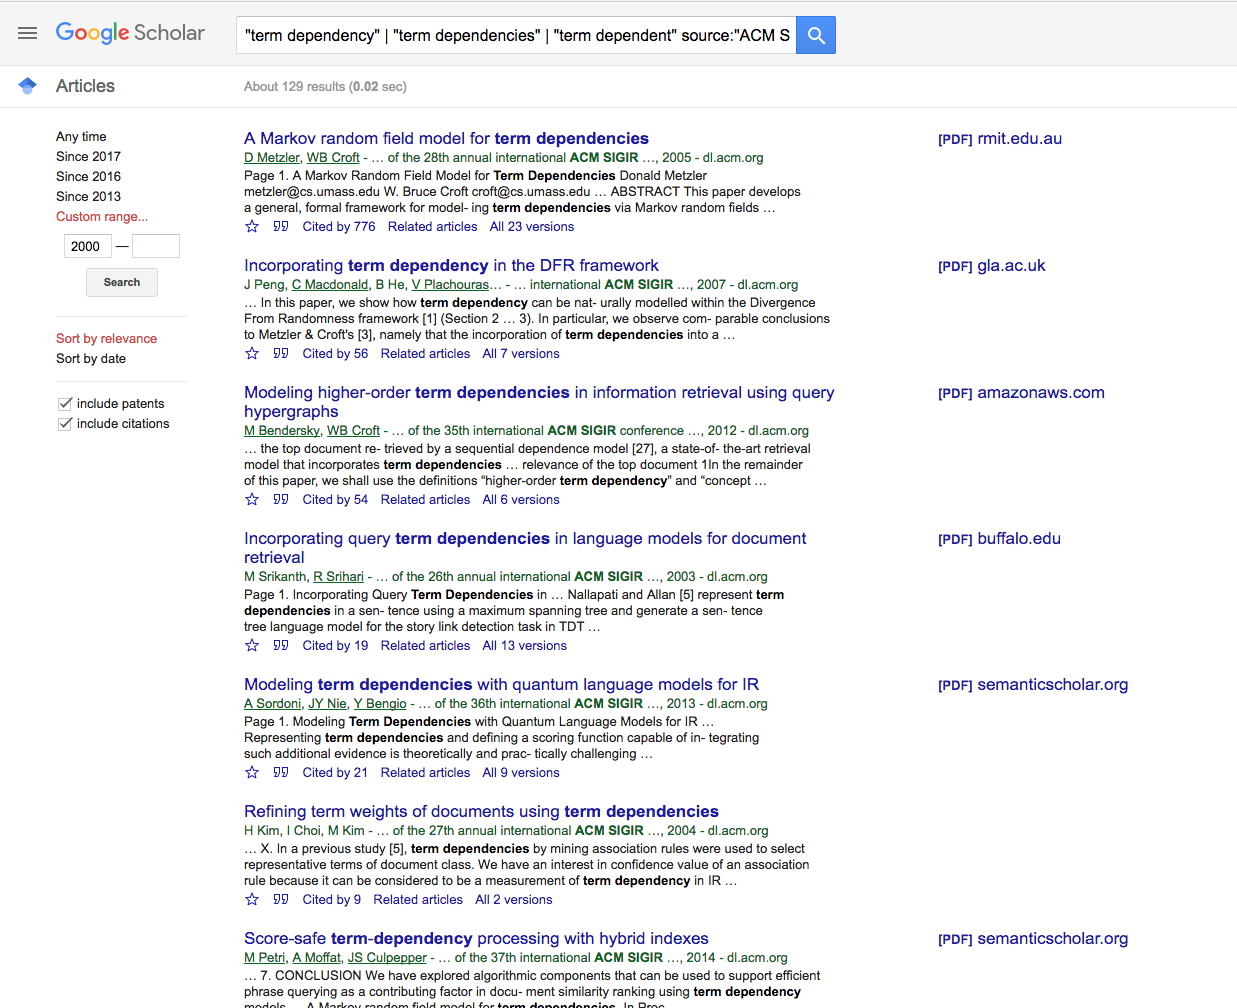
\includegraphics[scale=0.4]{sigir.png}
\caption{Google scholar results for term dependency articles later than 2000 for ACM SIGIR}
\label{fig:sigir}
\end{figure}

\clearpage

% =================================
% 5th question
% =================================

\section*{5}

\subsection*{Question}

\begin{verbatim}
11.11. Look at a sample of images or videos that have been 
tagged by users and separate the tags into three groups: 
those you think could eventually be done automatically
by image processing and object recognition, those you think would
not be possible to derive by image processing, and spam. Also 
decide which of the tags should be most useful for queries 
related to those images. Summarize your findings.
\end{verbatim}

\subsection*{Answer}

To answer this question I decided to use Instagram to find images tagged by users.
Instagram, much like Twitter, allows for users to tag photos and posts using a \# symbol.
Its apparent that many posts on these sites bring in spam tags to get higher views or for other reasons.

For this problem I first started with a base hashtag ``\#lamborghini'' and got a lot of unexpected results as shown in Figure \ref{fig:insta_results}.
Just from the top six results, only half of the results were lamborghini model cars.
You can tell just from these results that the non lamborghini tags were probably just spam tags.

When choosing one of the images from result page, such as Figure \ref{fig:bug}, its seen that the result is actually lamborghini was a spam tag for this image.
The tags used were:

\begin{itemize}
  \item Ferrari
  \item PaganiHuaryaBC
  \item pagani
  \item supercars
  \item fast
  \item speed
  \item london
  \item omg
  \item khk
  \item harrods
  \item city
  \item nightlife
  \item lamborghini
  \item astonmartin
  \item bugatti
  \item like4like
  \item likeforfollow
  \item followforfollow
  \item follow4follow
  \item rich
  \item wealth
  \item earth
  \item lifestyle
\end{itemize}

A majority of these tags would end up in spam.
There are, however, a few of the tags that could be derived from image processing such as: 
supercars, bugatti, and city.
If a image processing is done, assuming it is accurate, then the tags that address other types of cars, such as Ferrari, PaganiHuaryaBC, lamborghini, astonmartin, and paganic, should not be grouped together with the actual descriptors of this image.
Tags that could not be taken from image processing, or rather should not, are things like wealth and earth since the first one is opinionated and earth is too broad of a topic.
Tags such as likeforlike, follow4follow, omg, speed, wealth, and a few others, are more of spam tags for this image. 
The lamborghini tag itself is also considered spam for Figure \ref{fig:bug}, as the car isn't even a lamborghini.

The tags that would be most useful for queries would be the objects actually located inside the image.
For example, bugatti is a good descriptor of the car in the image as its exactly whats in the image and it is also considered a supercar.
However, if we search for supercar then we'll get much broader search results.
So if I had to choose tags from this image, I would probably only choose bugatti if I wanted concise results.
Of course there are many tags that could be used for recommendations based off of this tag, such as rich, city, or supercar that could be recommended to users. 


\begin{figure}[h]
\centering
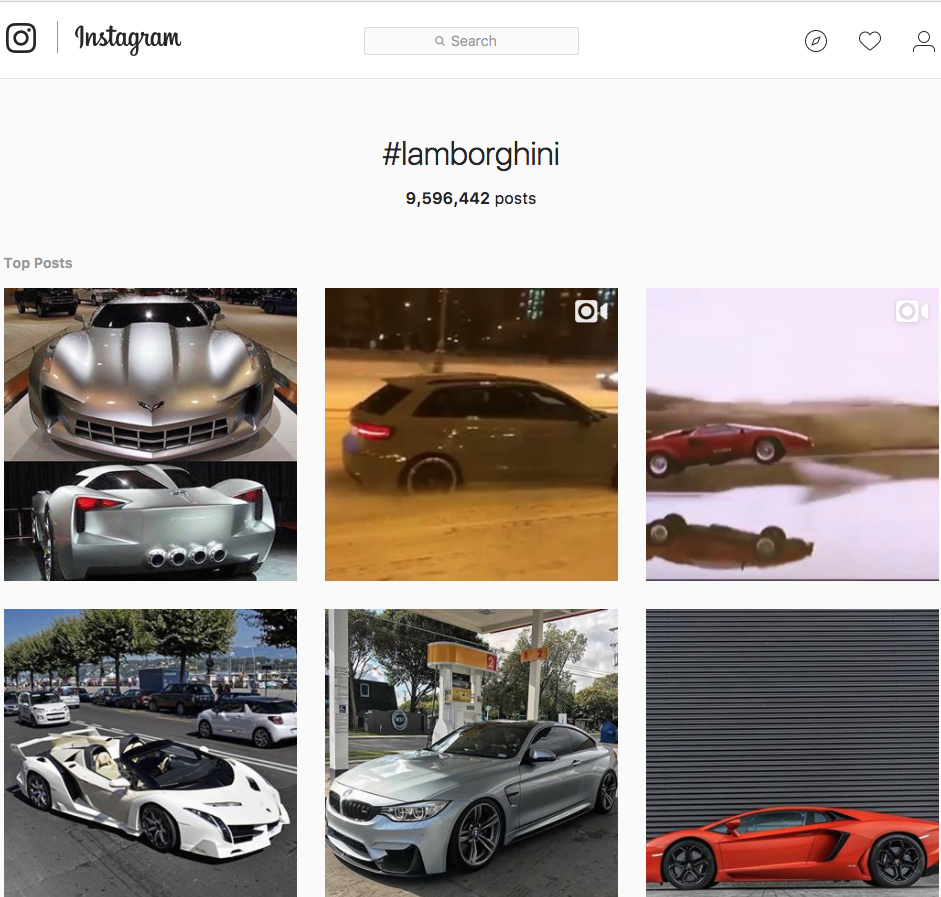
\includegraphics[scale=0.4]{insta_results.png}
\caption{Results page from Instagram}
\label{fig:insta_results}
\end{figure}

\begin{figure}[h]
\centering

\includegraphics[scale=0.4]{multi_class.png}
\caption{Selected result from Instagram for \#lamborghini tag}
\label{fig:bug}
\end{figure}


\clearpage


\clearpage


% =================================
% Bibliography
% =================================

\begin{thebibliography}{9}
\bibitem{github}
Atkins, Grant. ``CS734 Assignment 5 Repository'' Github. N.p., 15 December 2017. Web. 15 December 2017.\url{https://github.com/grantat/cs834-f17/tree/master/assignments/A5}.
\end{thebibliography}

\end{document}
